%%%%%%%%%%%%%%%%%%%% author.tex %%%%%%%%%%%%%%%%%%%%%%%%%%%%%%%%%%%
%
% sample root file for your "contribution" to a contributed volume
%
% Use this file as a template for your own input.
%
%%%%%%%%%%%%%%%% Springer %%%%%%%%%%%%%%%%%%%%%%%%%%%%%%%%%%


% RECOMMENDED %%%%%%%%%%%%%%%%%%%%%%%%%%%%%%%%%%%%%%%%%%%%%%%%%%%
\documentclass[graybox]{svmult}

% choose options for [] as required from the list
% in the Reference Guide

\usepackage{mathptmx}       % selects Times Roman as basic font
\usepackage{helvet}         % selects Helvetica as sans-serif font
\usepackage{courier}        % selects Courier as typewriter font
\usepackage{type1cm}        % activate if the above 3 fonts are
                            % not available on your system
%
\usepackage{makeidx}         % allows index generation
\usepackage{graphicx}        % standard LaTeX graphics tool
                             % when including figure files
\usepackage{multicol}        % used for the two-column index
\usepackage[bottom]{footmisc}% places footnotes at page bottom

\usepackage{qtree, bm, amsmath, amssymb, qtree, bm, multirow, textcmds, siunitx, mathrsfs, float, booktabs, color, soul}
\usepackage{natbib, setspace}
\usepackage{pdfpages} %To insert pdf pages
\usepackage[bb=boondox]{mathalfa}
\usepackage{tikz}
% see the list of further useful packages
% in the Reference Guide

\makeindex             % used for the subject index
                       % please use the style svind.ist with
                       % your makeindex program

%%%%%%%%%%%%%%%%%%%%%%%%%%%%%%%%%%%%%%%%%%%%%%%%%%%%%%%%%%%%%%%%%%%%%%%%%%%%%%%%%%%%%%%%%
%\textsc{\textsc{\bibliographystyle{natbb}
%
%\bibliography{References_HTSF}

\def\ba{\begin{pmatrix}\tilde{\vec{b}}\\ \tilde{\vec{a}}\end{pmatrix}}
\def\GH{\begin{pmatrix}\vec{G}\\ \vec{F}\end{pmatrix}}

\begin{document}

\title*{Hierarchical Forecasting}
% Use \titlerunning{Short Title} for an abbreviated version of
% your contribution title if the original one is too long
\author{Name of First Author and Name of Second Author}
% Use \authorrunning{Short Title} for an abbreviated version of
% your contribution title if the original one is too long
\institute{Name of First Author \at Name, Address of Institute, \email{name@email.address}
\and Name of Second Author \at Name, Address of Institute \email{name@email.address}}
%
% Use the package "url.sty" to avoid
% problems with special characters
% used in your e-mail or web address
%
\maketitle

\abstract*{TBC}


\section{Introduction}

The key macroeconomic indicators such as Gross Domestic Product (GDP), inflation and monetary policies which are used to study the behavior and performance of an economy as a whole are it self aggregates of various other components. 
For example, if we take the GDP growth, it is the aggregate of consumption, government expenditure, investments and net exports. These four components are again aggregates of some sub components. When we collect data for each of these individual variables over some time period, we will observe a collection of multiple time series that are bounded with some aggregation constraints. Thus the macroeconomic data are naturally forming cross sectional hierarchical time series. 

If the interest is on a single macroeconomic variable along different time granularities, then it can be considered as a temporal hierarchy. For example, suppose we have monthly consumer product index (CPI) of a particular country. The quarterly CPI is then the aggregate of corresponding monthly CPI of each quarter. Similarly the yearly CPI is the aggregate of quarterly CPI of each year. Hence it will form a temporal hierarchy. 

Macroeconomic forecasts are crucial for economic and business activities of any economy. Therefore this area of study has a long history in literature. Econometricians have developed various approaches for getting reliable economic forecasts using macroeconomic data. However, the information of aggregation structure in real data is limitedly used in literature. Moreover, having coherent forecasts will help the economists and policy makers for align decision making that impact for the whole economy. Therefore, our focus in this chapter is to introduce hierarchical forecasting methods for macroeconomic forecasting particularly for cross-sectional hierarchical data structures. 

Obtaining coherent forecasts are independent from the forecasting models. That means forecasters were given the freedom to use any reliable forecasting method to obtain the forecasts for individual series in the hierarchy. Getting coherent forecasts is a post-processing technique which ensures the aggregation properties are preserved in the forecasts.   \\


\textcolor{red}{briefly discuss the point forecasts as well as probabilistic forecasts in the sense of macroeconomic data  }

\begin{itemize}
	\item Importance of coherency
	\item Point forecasting
	\item Probabilistic forecasting
\end{itemize}

\section{GDP of Australia}

According to the Australian Bureau of Statistics (ABS), GDP of Australia is measured in three main approaches namely, Production, Income and Expenditure. Each of the three approaches naturally form a hierarchy according to the way data are collected and aggregated. Figures \ref{GDP_P_fig1}, \ref{GDP_I_fig1} and \ref{GDP_E_fig1} depict these hierarchies. In each hierarchy, the most aggregate level is denoted in gray whereas, the most disaggregate level is denoted in red. The intermediate levels are denoted in orange and blue. Levels denoted in orange continues to disaggregate further and these are separately depicted in different tree diagrams. Further, a description of each series in these hierarchies along with the series ID assigned by the ABS is given in the tables \ref{Tab: Income-hierarchy}, \ref{Tab:Expenditure-hierarchy-1}, \ref{Tab:Expenditure-hierarchy-2} and \ref{Tab:Expenditure-hierarchy-3} in appendix 1.
. 

GDP and its associated components are generally measured in different price indexes. \textit{Current price value} is one such price index which measures the sum of individual transaction values - quantity produced or sold multiplied by the unit price of a particular period. Alternatively, the production growth irrespective to the price change is measured by holding the price constant at a base year - referred to as \textit{constant price index} or by linking the period-to-period price indexes via an index formula - referred to as \textit{chain volume index} \citep{ABS2015}. Although the current prices are subjective to the changes of price in period-to-period, unlike chain volume indexes, these estimates satisfy the coherency of observed data. Therefore we consider the current prices of all series as the coherency is important in this study. 

We use seasonally unadjusted quarterly data ranging from 1984-Q4 to 2018-Q1. Since the current prices of quarterly series are not available for production approach, we consider only the income and expenditure approaches in our study. Further, the current price estimates of GDP is calculated by reflating the average chain volume estimates over three approaches by the implicit price deflator derived from the expenditure-based estimate. As a result, there exist a statistical discrepancy for GDP estimates in each approach \citep{ABS2018}. These were also included in the hierarchy in order to align with the coherency conditions in observed data. Furthermore, adjusting for seasonality in each series will deviate the aggregate constraints of the hierarchy. Thus we use seasonally unadjusted data to preserve coherency.


Following subsections will give a brief description of income and expenditure hierarchies.

\subsection{Income approach}

In the income approach, the GDP is measured by the aggregation of all income flows. That is the aggregation of all factor incomes  and the taxes less subsidies on production and imports at purchaser's price \citep{ABS2015}. Underline equation is given as, 
\begin{small}
	\begin{align*}
	GDP(I) &= \textit{Compensation of employees} + \textit{Gross operating surplus} + \textit{Gross mixed income}\\ &+ \textit{Taxes on production and imports} - \textit{Subsidies on production and imports}\\ &+ \textit{Statistical decrepency (I)}\\
	\end{align*}
\end{small}
Hierarchy shown in figure \ref{GDP_I_fig1} in appendix 1 reflects how these are further disaggregated. 

\subsection{Expenditure approach}

In the expenditure approach, the GDP is calculated as the aggregation of final consumption expenditure, gross fixed capital formation (GFCF), changes in inventories of finished goods, work-in-progress and raw materials and the value of exports less imports of the goods and services \citep{ABS2015}. Underline equation is, 

\begin{small}
	\begin{align*}
	GDP(E) &= \textit{Final consumption expenditure} + \textit{Gross fixed capital formation} + \textit{Changes in inventories}\\ &+ \textit{Exports of goods and services} - \textit{Imports of goods and services} + \textit{Statistical decrepency (E)}\\
	\end{align*}
\end{small}
Associated hierarchical structure is given in figure \ref{GDP_E_fig1}, \ref{GDP_E_fig2} and \ref{GDP_E_fig3} in appendix 1. 

Income and expenditure hierarchies consist 16 and 81 series respectively. All quarterly data for these series were obtained from the ABS and used to estimate coherent forecasts for Australian GDP along with its disaggregate components. In the following section we describe the hierarchical forecasting methods that we are using to get these forecasts. 

\section{Notations and preliminaries} 

This section discusses some preliminaries related to hierarchical time series. First let us start with introducing some notations. 

\begin{figure}[H]
	\begin{center}
		\leaf{AA} \leaf{AB} 
		\branch{2}{A}
		\leaf{BA} \leaf{BB}
		\branch{2}{B}
		\branch{2}{Tot}
		\qobitree
	\end{center}
	\caption{Two level hierarchical diagram}\label{fig1}
\end{figure}

Figure \ref{fig1} represents a two level cross sectional hierarchical time series, where the hierarchy is defined across time series for a particular time $t$. In this hierarchy, $Tot$ represents the most aggregate level series. We refer to this level as level~0 The observed value at a particular time $t$ of this series is denoted by $y_{Tot,t}$. $Tot$ is then disaggregated to $A$ and $B$ which lies in the level~1 of the hierarchy. Observed values of these at time $t$ is denoted by $y_{A,t}$ and $y_{B,t} $. Further $A$ and $B$ are disaggregated to $AA, AB$ and $BA, BB$ respectively. These series lies in the level~2 of the hierarchy and $t^\text{th}$ observations are denoted by $y_{AA,t}, y_{AB,t}, y_{BA,t}, y_{BB,t}$. Then $\vec{y}_t = [y_{Tot,t},y_{A,t}, y_{B,t},y_{C,t},y_{AA,t}, y_{AB,t}, y_{BA,t}, y_{BB,t}]'$ is a vector that consists all the observations of the hierarchy at time $t$. Moreover, $\vec{b}_t = [y_{AA,t}, y_{AB,t}, y_{BA,t}, y_{BB,t}]'$ is a vector consisting the observations of bottom level series at time $t$. $n$ and $m$ denote the number of total series in the hierarchy and the number of bottom level series respectively. Thus, $\vec{y}_t \in \mathbb{R}^n$ and $\vec{b}_t \in \mathbb{R}^m$. 

Due to the aggregation nature of the hierarchical time series we can write,
\begin{equation}
\vec{y}_t = \vec{Sb}_t,
\end{equation}
where $\vec{S}$ is a $(n \times m)$ constant matrix for a given hierarchical structure. For the hierarchy given in figure \ref{fig1}, 
\begin{equation}
\vec{S} = \begin{pmatrix} 
1& 1& 1& 1  \\ 
1& 1& 0& 0 \\   
0& 0& 1& 1 \\ 
& \multicolumn{2}{c}{I_4} &   
\end{pmatrix}. 
\end{equation} 
where $\vec{I}_4$ is a $4$-dimensional identity matrix.

Columns of $\vec{S}$ span the linear subspace of $\mathbb{R}^n$ for which all constraints hold. This subspace is also referred to as \textit{coherent subspace} and denoted by $\mathfrak{s}$. Pre-multiplying a vector in $\mathbb{R}^m$ by $\vec{S}$ will linearly transform that vector to another vector which lies in $\mathfrak{s}$. Therefore, although it is an $n$-dimensional vector, it actually lies in $\mathfrak{s}$. In earlier studies, $\vec{S}$ is also referred to as the ``summing matrix" since it aggregates the observations of bottom level to the corresponding upper levels.  


\section{Hierarchical point forecasting}

Efficient and accurate coherent point forecasting methods have been well studied and established in hierarchical literature over the past few decades. This section is devoted for a comprehensive discussion on these methodologies. 

\subsection{Coherent point forecasts}

Coherent forecasts preserve the aggregation structure of hierarchical time series. That is the forecasts of lower level series aggregates up to their corresponding upper level series of the hierarchy. In geometric language, the coherent forecasts lie in the coherent subspace $\mathfrak{s}$. Suppose $\breve{\vec{y}}_{t+h|t}$ consists point forecasts of all series in the hierarchy at time $t+h$ conditional on the past observations upto time $t$. Elements of $\breve{\vec{y}}_{t+h|t}$ are stacked in the same order as $\vec{y}_t$. Then, $\breve{\vec{y}}_{t+h|t}$ is said to be coherent  if $\breve{\vec{y}}_{t+h|t} \in \mathfrak{s}$. 

Let us consider the smallest possible hierarchy with two bottom level series, $A$ and $B$ that add up to the top level $Tot$. Suppose $\breve{\vec{y}}_{t+h|t}$ of this hierarchy is given by $\breve{\vec{y}}_{t+h|t} = [\breve{y}_{Tot,t+h|t},\breve{y}_{A,t+h|t}, \breve{y}_{B,t+h|t}]$. Due to the aggregation structure we have $\breve{y}_{Tot,t+h|t}=\breve{y}_{A,t+h|t}+\breve{y}_{B,t+h|t}$. This implies that, even though  $\breve{\vec{y}}_{Tot,t+h|t} \in \mathbb{R}^3$, the points actually lie in $\mathfrak{s}\subset \mathbb{R}^3$, which is a two dimensional subspace within $\mathbb{R}^3$ space. 

The most earlier studies on hierarchical literature involves forecasting series only in one layer of the hierarchy and then aggregate or disaggregate through the corresponding structure to get coherent forecasts. Let us briefly discuss about these traditional methods.  


\subsubsection{Bottom-up approach}

In bottom-up approach, forecasts of the lowest level series are first generated and these are  aggregated to get the forecasts at upper levels of the hierarchy \citep{dunn1976}. That is, considering the hierarchy given in Figure \ref{fig1}, first the forecasts for series $AA, AB, BA$ and $BB$ are obtained. Then the forecasts of series $A$ is obtained by simply adding the forecasts of $AA$ and $AB$. Similarly the forecasts of $B$ is obtained by adding the forecasts of $BA$ and $BB$. The forecasts of  $Tot$ series is then the aggregation of $A$ and $B$ which in turn the sum of forecasts of $AA, AB, BA$ and $BB$. 

In terms of notations, let $\hat{\vec{b}}_{t+h|t} \in \mathbb{R}^m$ consists $h$-step ahead forecasts of the bottom levels series. i.e. $\hat{\vec{b}}_{t+h|t} = (\hat{{y}}_{AA,t+h|t}, \hat{{y}}_{AB,t+h|t}, \hat{{y}}_{BA,t+h|t}, \hat{{y}}_{BB,t+h|t}),$ where, $\hat{{y}}_{i,t+h|t}$ is the $h$-step ahead forecasts of $i^\text{th}$ series. Then, the bottom-up forecasts are given by,
\begin{equation}\label{eq:03}
\breve{\vec{y}}^{BU}_{t+h|t}=\vec{S\hat{\vec{b}}}_{t+h|t}.
\end{equation}

Even though this method looks easy to construct, it is less reliable. In fact, bottom up approach provides accurate forecasts only if the bottom level series of the hierarchy are accurately forecast. However, if the bottom level series are highly volatile or too noisy, then they are challenging to forecast. Thus the bottom-up approach would produce unreliable point forecasts. 

\subsubsection{Top-down approach}

In contrast to the bottom-up method, the top-down approach involves forecasting the most aggregated series first and then disaggregating these forecasts down the hierarchy.  

In general, all top-down forecasts can be written as, 

\begin{equation}\label{eq:04}
\breve{\vec{y}}^{TD}_{t+h|t}=\vec{S}\hat{y}_{Tot, t+h|t}\vec{p},
\end{equation}
where $\vec{p} = (p_1,...,p_m)$ is a $m$ dimensional vector of proportions consisting the disaggregation proportions of the bottom level series with respect to the top level series. 

Usually, these proportions are calculated based on observed data, which is referred to as historical proportions. \cite{gross1990} provide a comprehensive summary on using historical proportions in this context. Commonly there are two approaches of using historical proportions. One is to use the average of historical proportions of desired bottom level series relative to the total series. That is, the historical proportion of $j^{\text{th}}$ series is given by, 

\begin{equation}
p_j = \frac{1}{T} \sum_{t=1}^{T}\frac{Y_{j,t}}{Y_{tot,t}}.
\end{equation}

The second approach is to use the proportion of average of the bottom level series $y_{j,t}$ over the time $t=1,...,T$ relative to that of the total series $y_{Tot,t}$. i.e.

\begin{equation}
p_j = \frac{\frac{1}{T}\sum_{t=1}^{T}y_{j,t}}{\frac{1}{T}\sum_{t=1}^{T}y_{Tot,t}}
\end{equation}

However, the largest limitation of these approaches is that its inability to reflect the characteristics of individual series such as trends, seasonality or other special events, in the forecasts of disaggregate levels. This will mainly effect the hierarchies with series having different patterns in different levels.  

To overcome this limitation, \cite{athanasopoulos2009} introduced a new top-down approach which disaggregate the top level forecasts according to the proportions of forecasts rather than historical proportions. They found that their method outperforms the conventional top-down approach through an empirical application. 

Recently, \cite{Mircetic2017} proposed a modified approach to the conventional top-down methods, which involves forecasting $h$-step ahead proportions of bottom level series relative to the top level series. That is, let the ratio between the $j^\text{th}$ bottom level series and the top level series is given by, $p_{j,t}=y_{j,t}/y_{Tot,t}$, for $t=1,...,T$. Then this series of proportions will be forecast for the $h$-step ahead period, which is denoted by $\hat{p}_{j,T+h|T}$. These proportions will be then used as the disaggregate proportions to construct coherent top-down forecasts. Thus giving the elements of vector $\vec{p}$ as,

\begin{equation}
p_j = \hat{p}_{j,T+h|T}.
\end{equation}   

This approach is much reliable, since it calculates the proportions as a function of time, rather than using the simple averages in traditional top-down methods. 

As shown by \cite{hyndman2011}, top-down methods are adding a bias component to each disaggregate level. Therefore, all these top-down approaches are producing biased forecasts even if the top level base forecasts are unbiased.  


\subsubsection{Middle-out approach}

A compromise between these two approaches is the middle-out method which entails forecasting each series of a selected middle level in the hierarchy and then forecasting upper levels by the bottom-up method and lower levels by the top-down method.\\
Since this is a hybrid approach of bottom-up and top-down approaches it still remains the limitations of those two. 


\subsection{Point forecast reconciliation}

The common limitation of traditional hierarchical forecasting methods is that the loss of structural information of individual series, as it precisely forecasting only one level of series in the hierarchy.  

As an alternative to these traditional methods, \citet{hyndman2011} proposed to utilize the information from all levels of the hierarchy to obtain coherent point forecasts in  a two stage process. In the first stage, the forecasts of all series are independently obtained by fitting univariate models for individual series in the hierarchy. It is very unlikely that these forecasts are coherent. Thus in the second stage, these forecasts are optimally combined through a regression model to obtain coherent forecasts. This second step is referred to as ``reconciliation'' since it takes a set of incoherent forecasts and revises them to be coherent.

This was the first study to introduced the concept of forecast reconciliation in the hierarchical literature. Since this approach starts from the individual forecasts, it uses all the relevant information from the hierarchy in producing coherent forecasts. Thus improves the drawbacks from traditional approaches, in particularly the loss of information. Further reconciliation step is independent from the initial step of getting individual forecasts for all series in the hierarchy. Therefore, forecasters are given the choice to use the best possible forecasting method to get forecasts for all individual series. However the unbiasedness property of the reconciled forecasts will be preserved only if all the individual forecast are unbiased. We will discuss this property as we follows in this section.  

Suppose we fit univariate time series models for all series based on data upto time $t$ and obtained $h$-step ahead forecasts. These forecasts are then formed in a vector $\hat{\vec{y}}_{t+h|t}$ by stacking the forecasts at each node in the same order as $\vec{y}_{t}$. Since these do not satisfy the aggregate constraints of the hierarchy, they are often referred to as ``incoherent'' forecasts. In some texts these also referred to as ``base'' forecasts. 

Reconciliation of $\hat{\vec{y}}_{t+h|t}$ involves, revising these forecasts such that they lies in the coherent subspace. We do this by projecting $\hat{\vec{y}}_{t+h|t}$ onto the coherent subspace through the projection matrix $\vec{SG}$ for any $m\times n$ matrix $\vec{G}$. Let $\tilde{\vec{y}}_{t+h|t}$ be a vector that contains reconciled forecasts. Then, 

\begin{equation} \label{eq:08}
\tilde{\vec{y}}_{t+h|t}=\vec{S}\vec{G}\hat{\vec{y}}_{t+h|t}.
\end{equation}

Pre-multiplying the incoherent forecasts, $\hat{\vec{y}}_{t+h|t}$ by $\vec{G}$ will maps $\hat{\vec{y}}_{t+h|t}$ to the $\mathbb{R}^m$ space. This will gives the reconciled forecasts of bottom level series of the hierarchy. Next these forecasts will be mapped to the coherent subspace by the pre-multiplication of $\vec{S}$ matrix. 

It is also worth discussing the unbiased property of these reconciled point forecasts. Let us assume the incoherent forecasts, $\hat{\vec{y}}_{t+h|t}$ are unbiased. That is, $E_{1:t}(\hat{\vec{y}}_{t+h|t})=\umu_{t+h|t}$ where $\umu_{t+h|t} = E_{1:t}[\vec{y}_{t+h}|\vec{y}_1,...,\vec{y}_t]$ is the true mean of the hierarchy. Here the expectation is taken over the observed data upto time $t$. Then for any $\vec{G}$ such that $\vec{SGS}=\vec{S}$ produces unbiased reconciled forecasts (\cite{hyndman2011}). Further any reconciliation method that define through a projection $\vec{SG}$ will always produce unbiased reconciled forecasts given that the incoherent forecasts are unbiased \citep{Gamakumara2018}. \\

\subsection{Existing point forecast reconciliation methods}

Structures of $\vec{G}$ define different reconciliation methods. First let us reconsider the traditional bottom up approach. Suppose we have a set of incoherent forecasts, $\hat{\vec{y}}_{t+h|t}$. Following equation (\ref{eq:03}), we can write, $\breve{\vec{y}}^{BU}_{t+h|t}=\vec{S}\begin{pmatrix}
0_{(m \times n-m)} & \vec{I}_m
\end{pmatrix}\vec{\hat{y}}_{t+h|t}$. where $\bm{G}=\begin{pmatrix}
0_{(m \times n-m)} & \bm{I}_m
\end{pmatrix}$. Since $\vec{SG}$ in this case is a projection matrix, bottom-up method also produces unbiased coherent forecasts. However, it is not always a preferred approach since it ignores the information from aggregate levels of the hierarchy.

\subsubsection{OLS reconciliation}

Intuitively, the reconciliation starts with a set of incoherent forecasts, $\hat{\vec{y}}_{t+h|t}$. \cite{hyndman2011} proposed to optimally combine these incoherent forecasts through the following regression model.  
\begin{equation} \label{eq:09}
\hat{\vec{y}}_{t+h|t} = \vec{S\ubeta}_{t+h|t} + \vec{\varepsilon}_{t+h|t},
\end{equation}
where $\vec{\ubeta}_{t+h|t}=E[\vec{b}_{t+h}|\vec{b}_1,.....,\vec{b}_t]$ is the unknown conditional mean of the bottom level series at time $t+h$ and $\vec{\varepsilon}_{t+h|t}$ is the reconciliation error with mean zero and variance $\vec{V}$. The ordinary least squares (OLS) solution for the above regression model gives, 
\begin{equation} \label{eq:10}
\vec{\hat{\ubeta}}_{t+h|t} = (\vec{S}'\vec{S})^{-1}\vec{S}'\hat{\vec{y}}_{t+h|t},
\end{equation}
and thus giving the reconciled forecasts, 
\begin{equation} \label{eq:11}
\tilde{\vec{y}}_{t+h|t} = \vec{S\hat{\ubeta}}_{t+h|t} = \vec{S}(\vec{S}'\vec{S})^{-1}\vec{S}'\hat{\vec{y}}_{t+h|t}.
\end{equation}

$(\vec{S}'\vec{S})^{-1}\vec{S}'$ is the corresponding $\vec{G}$ matrix in OLS reconciliation. Further in this reconciliation, the incoherent forecasts are orthogonally projected to the coherent subspace $\mathfrak{s}$. Thus it will minimises the Euclidean distance between $\hat{\vec{y}}_{t+h|t}$ and $\tilde{\vec{y}}_{t+h|t}$. 

In a later study by \cite{Wickramasuriya2018} showed that the variance covariance matrix of the reconciliation error, $\vec{\varepsilon}_{t+h|t}$ in the above regression model is not identifiable and thus the GLS solution that \cite{hyndman2011} proposed for the same model is unattainable. 


\subsection{MinT reconciliation}

As an improved work of \cite{hyndman2011}, \cite{Wickramasuriya2018} find an unique analytical solution for producing unbiased reconciled point forecasts, by minimising the sum of variances of reconciled forecast errors. Suppose the variance of $h$-step ahead base forecast errors is denoted by, $Var(\vec{y}_{t+h} - \hat{\vec{y}}_{t+h|t}|\vec{y}_1,...,\vec{y}_t) := \vec{W}_{t+h|t}$. \cite{Wickramasuriya2018} first showed that the variance of the reconciled forecast errors, i.e $Var(\vec{y}_{t+h} - \tilde{\vec{y}}_{t+h|t}|\vec{y}_1,...,\vec{y}_t) := \tilde{\vec{W}}_{t+h|t}$ is given by,
\begin{equation} \label{eq:12}
\tilde{\vec{W}}_{t+h|t} = \vec{SG}\vec{W}_{t+h|t} \vec{G}'\vec{S}'
\end{equation}
for any choice of $\vec{G}$. Then they minimize the trace of $\tilde{\vec{W}}_{t+h|t}$ with respect to $\vec{SGS=S}$ to obtain an optimal $\vec{G}$. By imposing the unbiased constraint they ensure that the resulting reconciled forecasts are unbiased. The closed form solution to this minimization problem is given by,
\begin{equation} \label{eq:13}
\vec{G} = (\vec{S}'{\vec{W}}^{-1}_{t+h|t}\vec{S})^{-1}\vec{S}'{\vec{W}}^{-1}_{t+h|t},
\end{equation}
and they named this as MinT approach. The reconciled point forecasts are then given by,
\begin{equation} \label{eq:14}
\tilde{\vec{y}}_{t+h|t} = \vec{SG}\hat{\vec{y}}_{t+h|t} = \vec{S}(\vec{S}'{\vec{W}}_{t+h|t}^{-1}\vec{S})^{-1}\vec{S}'{\vec{W}}_{t+h|t}^{-1}\hat{\vec{y}}_{t+h|t}.
\end{equation}\\

In terms of projections, MinT is doing an oblique projection of $\hat{\vec{y}}_{t+h|t}$ onto the coherent subspace $\mathfrak{s}$. Further in terms of distances, MinT minimises the Mahalonobis distance between $\hat{\vec{y}}_{t+h|t}$ and $\tilde{\vec{y}}_{t+h|t}$ as proven by \cite{Wickramasuriya2018}.   

Unlike OLS, MinT reconciliation imposes the correlation structure of the whole hierarchy to reconcile the point forecasts. However, estimating ${\vec{W}}_{t+h|t}$ is challenging. \citet{Wickramasuriya2018} discussed possible alternative estimates of ${\vec{W}}_{t+h|t}$ and how these lead to different $\vec{G}$ matrices. Let us briefly summarise these below.

Suppose we have the in-sample data up to time $T$. Since the variance covariance matrix of $1$-step ahead incoherent forecast errors are approximately proportional to that of $h$-step ahead incoherent forecasts errors, we have $\vec{W}_{T+h|T} = \alpha\vec{W}_{T+1|T}$ where $\alpha>0$. Therefore, to estimating ${\vec{W}}_{T+h|T}$ is sufficient to determine $\vec{G}$. If ${\vec{W}}_{T+1}$ is approximated by an identity matrix, then $\vec{G}$ in (\ref{eq:14}) collapses to OLS reconciliation. Following are a few other estimates for ${\vec{W}}_{T+1}$. 

\subsection*{MinT(Sample)}

The unbiased sample variance covariance matrix of 1-step ahead incoherent forecast errors can be used as the most reasonable estimator for ${\vec{W}}_{T+1|T}$. That is, 
\begin{equation}\label{eq:15}
\hat{\vec{W}}_{T+1|T} = \frac{1}{T}\sum_{t=1}^{T}\hat{\vec{e}}_{t+1}\hat{\vec{e}}'_{t+1},
\end{equation}
where $\hat{\vec{e}}_{t+1} = \vec{y}_{t+1}-\hat{\vec{y}}_{t+1|t}$ for $t=1,...,t-1$,  consists the 1-step ahead insample forecast errors. 


The resulting $\vec{G}$ matrix is referred to as MinT(Sample). This estimator is performing well in small hierarchies. However for the hierarchies with large dimensions, especially when $m>T$, this causes singularity problems. 

\subsection*{MinT(Shrink)}

Another alternative estimator for ${\vec{W}}_{T+1|T}$ is a shrinkage estimator, which is apparently useful in large dimensional hierarchies. This estimator is given by,
\begin{equation} \label{eq:16}
\hat{{\vec{W}}}_{T+1|T}^{shr} = \tau\hat{{\vec{W}}}_{T+1|T}^D + (1-\tau)\hat{{\vec{W}}}_{T+1|T},
\end{equation}
where $\hat{{\vec{W}}}_{T+1|T}^D$ is a diagonal matrix comprising diagonal entries of $\hat{{\vec{W}}}_{T+1|T}$ and 
$$\tau = \frac{\sum_{i \ne j}\hat{Var}(\hat{r}_{ij})}{\sum_{i \ne j}\hat{r}_{ij}^2}$$ is a shrinkage parameter proposed by \citet{schafer2005} where, $\hat{r}_{ij}$ is the $ij$-th element of sample correlation matrix.  In this estimation, the off-diagonal elements of 1-step ahead sample covariance matrix will be shrunk to zero depending on the sparsity.

\subsection*{WLS}

If ${\vec{W}}_{T+1|T}$ is approximated by a diagonal matrix with diagonal elements being the variances of incoherent forecast errors, then the resulting reconciliation is referred to as WLS reconciliation. This was first proposed by \cite{Hyndman2016} with reference to the regression model introduced in \cite{hyndman2011}. However a proper theoretical justification for the WLS reconciliation is given through MinT solution.

\subsection{GTOP reconciliation}

\cite{VanErven2015a} proposed to use a game theoretical approach to produce reconciled forecasts that are at least as good as incoherent forecasts. Initially starting with the best possible incoherent forecasts, they show that the sum of weighted squared loss of these incoherent forecasts will never be less than that for the reconciled forecasts.

This approach does not require unbiasedness assumption on incoherent forecasts and it allows forecasters to choose the best possible incoherent forecasts without depending on any assumptions. However this method doesn't guarantee to produce unbiased reconciled forecasts. Further, there is no closed form solution to this approach and thus would result a high computational cost in producing reconciled forecasts for large scale hierarchies.\\ 


Any reconciliation approach via projections such as MinT are preferred as they improve these limitations in the GTOP method. Nevertheless, they guarantee to produce coherent forecasts that are at least as good as incoherent forecasts (\cite{Wickramasuriya2018}, \cite{Gamakumara2018}). 


Another important feature of hierarchical time series is that they often consist of thousands or millions of individual series and thus imposes computational challenges in implementing any forecasting solutions. The MinT reconciliation method was further generalized to handle these constraints and to scale to large hierarchies by \cite{Wickramasuriya2018}. 


\section{Hierarchical probabilistic forecasting}

Point forecasts are limited because they provide no indication of forecast uncertainty. Providing prediction intervals helps \citep{Shang2017a}, but a richer description of forecast uncertainty is obtained by estimating the entire forecast distribution. These are often called ``probabilistic forecasts'' \citep{Gneiting2014}. For example, \citet{McSharry2005} produced probabilistic forecasts for electricity demand, \citet{BenTaieb2017} for smart meter data, \citet{Pinson2009} for wind power generation, and \citet{Gel2004}, \citet{Gneiting2005a} and \citet{Gneiting2005} for various weather variables.

Even though the point forecasts in hierarchical time series is well studied and having an established literature, the hierarchical probabilistic forecasting is still an emerging area of interest. There's is only a few studies in published literature. The uncertainly around $\vec{y}_{t+h|t}$ is referred to as the probabilistic forecasts in hierarchical time series. Due to the aggregation nature of the data, these should also lie in the coherent subspace $\mathfrak{s}$. If so, we call them as coherent probabilistic forecasts.    

\cite{Taieb2017} defined the coherent probabilistic forecasts in terms of convolution. That is, the predictive distributions of a hierarchy is said to be coherent, if the convolution of forecast distributions of disaggregate series is equal to the forecast distribution of the corresponding aggregate series. Based on this, they proposed an algorithm to produce coherent probabilistic forecasts and applied it to UK electricity smart meter data. 

Analogous to point forecast reconciliation, we can reconcile the forecast distributions to get coherent probabilistic forecasts. This will start with an incoherent forecast distribution of the whole hierarchy which was obtained by gathering all information available, and then projecting that to the coherent subspace similar in the point forecasting case. Geometric intuition behind the probabilistic forecast reconciliation is discussed in \cite{Gamakumara2018}. 

\subsection{Probabilistic forecast reconciliation in the Gaussian framework}

Suppose we have a set of hierarchical time series where each realisation follows a multivariate Guassian distribution. i.e., $\vec{y}_T \sim \mathscr{N}(\vec{\mu}_T, \Sigma_T)$ where both $\vec{\mu}_T$ and $\Sigma_T$ lives in the coherent subspace $\mathfrak{s}$ due to the aggregation structure of the hierarchy. We are interested in estimating the predictive Gaussian distribution of $\vec{Y}_{T+h}| \vec{\mathscr{I}}_T$ where $\vec{\mathscr{I}}_T= \{\vec{y}_1,\vec{y}_2,\dots.,\vec{y}_T\}$, which should also lives in $\mathfrak{s}$. Since Gaussian distributions are uniquely characterised by the first two moments, it is sufficient to have the mean and variance forecasts to get the Gaussian predictive distributions of the hierarchy.

Assume we have fit the time series models for each series of the hierarchy by considering all the available information. Using these fitted models we can estimate the means and variance forecasts of the hierarchy which are denoted by $\vec{\hat{\mu}}_{T+h}$ and $\hat{\Sigma}_{T+h}$ respectively. Each element in $\vec{\hat{\mu}}_{T+h}$ corresponds to the mean forecast of each series in the hierarchy and these elements are stacked in the same order as $\vec{y}_t$. Similarly $\hat{\Sigma}_{T+h}$ contains variances and covariances of all series in the hierarchy. One can either fit univariate models for each individual series of the hierarchy or fit multivariate models by considering the correlation structure of the series for getting these forecasts. However as long as the aggregation structure is not imposed, it is very unlikely that these forecasts will be coherent. Thus it comes to the point of reconciliation. 

Reconciling Gaussian forecast distribution is all about reconciling the incoherent means and variance of forecasts. That is, the reconciled Gaussian distribution is given by $\mathscr{N}(\vec{\tilde{\mu}}_{T+h}, \tilde{\Sigma}_{T+h})$, where, 

\begin{equation}\label{eq:17}
\vec{\tilde{\mu}}_{T+h} = \vec{SG}\vec{\hat{\mu}}_{T+h},
\end{equation} 
and
\begin{equation}\label{eq:18}
\tilde{\Sigma}_{T+h} = \vec{SG}\hat{\Sigma}_{T+h}\vec{G'S'}.
\end{equation} 

A more rigorous explanation about deriving these equations can be found in \cite{Gamakumara2018}. Depending on the choice of $\vec{G}$ we will get different Gaussian forecast distributions. The same choices of $\vec{G}$ matrices that has been used in the point forecasting case can be used in reconciling Gaussian forecast distributions. It is also worth mentioning that, due to the aggregation constraints, the distributions lies in $\mathfrak{s}$, which is a lower dimensional subspace of $\mathbb{R}^n$. Therefore, these reconciled Gaussian distributions are degenerate. 


\subsection{Probabilistic forecast reconciliation in the non-parametric framework}

In many applications it may not reasonable to assume parametric forecasting distributions. Therefore, non-parametric approaches has been widely used for probabilistic forecasts in different disciplines. For example, ensemble forecasting in weather applications (\cite{Gneiting2005}, \cite{Gneiting2014}, \cite{Gneiting2008}), bootstrap based approaches (\cite{Manzan2008}, \cite{Vilar2013}). 

Non-parametric approaches are also important in hierarchical forecasting as in most applications they have millions of time series which are often difficult to assume parametric distributions. Further, for data with heavy tails, it is often misleading to assume Gaussianity. The algorithm introduced by \cite{Taieb2017} is also a non-parametric approach as it does not make any distributional assumptions. They first generate, a sample from the bottom level predictive distribution, and then aggregate to obtain coherent probabilistic forecasts of the upper levels of the hierarchy. Initially they use MinT algorithm to reconcile the means of the bottom level forecast distributions, and then a copula-based approach is employed to model the dependency structure of the hierarchy. Resulting multi-dimensional distribution is used to generate the empirical forecast distributions for all bottom-level series which are then aggregated to obtain the empirical forecast distribution for the entire hierarchy. Although the means of forecast distributions are reconciled, the predictive distributions were obtained through a bottom-up based approach. Therefore this approach is not a reconciliation method as it does not use all the information from the hierarchy when producing coherent probabilistic forecasts. 

\cite{Jeon2018} is the only existing study that does reconciliation in probabilistic hierarchical forecasts. This method is based on cross-validation and it also does not assume any parametric distributions for predictive densities. However they applied this method particularly for temporal hierarchies. 

\cite{Gamakumara2018} discussed that reconciling the draws from incoherent forecast distribution will give draws from a reconciled forecast distribution. Employing this fact, we introduce a novel method based on a bootstrap approach. This involves a two steps process. In the first step we obtain possible sample paths from the incoherent forecast distributions. This follows by the reconciliation step which projects each sample path to the coherent subspace. These steps will be discussed in detail below. 

\subsection*{Step 1: Obtaining incoherent probabilistic forecasts}

Suppose we fit univariate time series models for the series at each node in the hierarchy, by using past observations up to time $T$. Using these fitted models, we can generate $h$ step ahead future sample paths for each node, by conditioning on past observations. In order to capture the dependency structure of the hierarchy, we incorporate bootstrapped training errors from the fitted models. That is, let $\varGamma_{(T \times n)}=(\vec{e}_1,\vec{e}_2,.....,\vec{e}_T)'$ denote the in-sample residual matrix where, $\vec{e}_t=\vec{y}_t-\hat{\vec{y}}_t$ is a vector that consists of residuals in each node at time $t$ and stacked in the same order as $\vec{y}_t$. $\varGamma$ is also referred to as the matrix of in-sample errors. Then we block bootstrap a sample of size $h$ from $\varGamma$, and these bootstrapped errors will be incorporated as the error series for simulating future paths. Taking block bootstrapped in-sample errors in generating future paths will implicitly model the dependency structure of the hierarchy. These simulated future sample paths will be then formed in a vector $\hat{\vec{y}}_{T+h|T}^b$ by stacking the sample paths of each node in the same order as $\vec{y}_t$. As such we generate a sample of $N$ future paths for the hierarchy. We can denote this sample by a $(N \times n)$ matrix $\hat{\vec{Y}}^b_{T+h|T}$ where, 

\begin{equation} \label{eq:19}
\hat{\vec{Y}}^b_{T+h|T}=\begin{pmatrix}
\hat{\vec{y}}_{1,T+h|T}^b\\
\hat{\vec{y}}_{2,T+h|T}^b\\
\vdots\\
\hat{\vec{y}}_{N,T+h|T}^b
\end{pmatrix}.
\end{equation}

Although the dependency structure of the hierarchy is captured through the bootstrap in-sample errors, the aggregation structure will not be reflected through these sample paths. Therefore, these future paths are incoherent and thus considered as a possible sample from the incoherent probabilistic forecast distribution of the hierarchy.

\subsection*{Step 2: Reconciling future sample paths}

The second step is to project these sample paths to the coherent subspace. Then we get a set of reconciled future paths which form a possible sample from the reconciled probabilistic forecast distribution. Similar to the projection used in the point forecast reconciliation, we project each sample path through the projection $\vec{SG}$. Then we get, 

\begin{equation} \label{eq:20}
\tilde{\vec{y}}_{i,T+h}^b = \vec{SG}\hat{\vec{y}}_{i,T+h}^b, \quad i = 1, ..., N
\end{equation}
and let
\begin{equation}\label{eq:21}
\tilde{\vec{Y}}^b_{T+h|T}=\begin{pmatrix}
\tilde{\vec{y}}_{1,T+h|T}^b\\
\tilde{\vec{y}}_{2,T+h|T}^b\\
\vdots\\
\tilde{\vec{y}}_{N,T+h|T}^b
\end{pmatrix}
\end{equation}
where, $\tilde{\vec{y}}_{i,T+h}^b \in \mathfrak{s}$ denote a $h$-step-ahead reconciled future paths for $i=1,...,N$. $\tilde{\vec{Y}}^b_{T+h|T}$ form an empirical coherent forecast distribution of the hierarchy that lies in the coherent subspace $\mathfrak{s}$. As we discussed in point forecast reconciliation methods, different estimates of $\vec{G}$ provide alternative estimates of reconciled future paths. We can also obtain bottom-up based future paths by simply aggregating the future paths of bottom level series for their respective upper levels. This is referred to as bottom-up future paths. Even though the bottom-up approach generates coherent probabilistic forecasts, it cannot be considered as a reconciliation method since it use only half of the information.

 
\section{Evaluation}

In this section we briefly discuss the methods that we use to measure the forecast accuracy of hierarchical forecasts. 

\subsection{Point forecast evaluation}

Any existing point forecast evaluation method can be used to evaluate the accuracy of hierarchical point forecast. We are mainly using Mean Squared Error (MSE) and Mean Absolute Scaled Error (MASE) in our empirical application. Mathematical expression for these measures are given below. 

\begin{equation}\label{eq:22}
MSE = mean(e^2_{t+h}),
\end{equation}
and
\begin{equation}\label{eq:23}
 MASE = mean(q_{t+h}),
\end{equation}
where $q_{t+h} = \frac{e_{t+h}}{\frac{1}{T-m}\sum_{j=m+1}^{T}|y_j - y_{j-m}|}$. Further $e_{t+h}$ is the forecast error, which is the difference between forecast and realisation.

MSE is a scaled dependent measure. Therefore to compare series in different scales or with different units, MASE is preferred. For more details on different point forecast accuracy measures refer to \cite{hyndman2018forecasting}. 
  
\subsection{Probabilistic forecast evaluation}

Forecast accuracy of probabilistic forecasts can be evaluated using scoring rules \cite{Gneiting2014}. Scoring rules provides a summary measurement based on the relationship between realisation and the forecast distribution. However, not all scoring rules are applicable for hierarchical probabilistic forecast evaluation. An comprehensive discussion on this can be found in \cite{Gamakumara2018}.  

Since the whole forecast distribution of the hierarchy is a multivariate distribution, the forecast accuracy should also be assessed in the multivariate framework. Therefore using multivariate scoring rules is helpful. Energy score \citep{Gneiting2008} and variogram scores \citep{SCHEUERER2015} are the mainly using multivariate scoring rules in hierarchical framework. Further, multivariate log score \citep{Gneiting2007} can also be used for evaluating parametric forecast distributions. The mathematical expressions for these are given table \ref{table:scoringrules}. 

\begin{table}[!b]
	\caption{Scoring rules to evaluate multivariate forecast densities. $\breve{\vec{y}}_{T+h}$ and $\breve{\vec{y}}^*_{T+h}$ be two independent random vectors from the coherent forecast distribution $\breve{\vec{F}}$ with the density function $\breve{\vec{f}}(\cdot)$ at time $T+h$ and $\vec{y}_{T+h}$ is the vector of realizations. Further $\breve{Y}_{T+h,i}$ and $\breve{Y}_{T+h,j}$ are $i$th and $j$th components of the vector $\breve{\vec{Y}}_{T+h}$. Moreover, the variogram score is given for order $p$ where, $w_{ij}$ are non-negative weights.}\label{table:scoringrules}
	\centering\small\setstretch{1.3}
	\begin{tabular}{@{}lp{8.1cm}}
		\toprule
		\textbf{Scoring rule}  & \textbf{Expression}           \\
		\midrule
		\text{Log score}       &
		$\text{LS}(\breve{\bm{F}},\bm{y}_{T+h}) = -\log {\breve{\bm{f}}(\bm{y}_{T+h})}$ \\\\[-0.2cm]
		\text{Energy score}    &
		$\text{eS}(\breve{\bm{Y}}_{T+h},\bm{y}_{T+h}) =
		E_{\breve{\bm{F}}}
		\|\breve{\bm{Y}}_{T+h}-\bm{y}_{T+h}\|^\alpha -$ \par\hfill
		$\frac{1}{2}E_{\breve{\bm{F}}}\|\breve{\bm{Y}}_{T+h}-\breve{\bm{Y}}^*_{T+h}\|^\alpha$, \,\, $\alpha \in (0,2]$ \\\\[-0.2cm]
		\text{Variogram score} &
		$\text{VS}(\breve{\bm{F}}, \bm{y}_{T+h}) =
		\sum\limits_{i=1}^{n}
		\sum\limits_{j=1}^{n}
		w_{ij}\Big(|y_{T+h,i} - y_{T+h,j}|^p -$ \par\hfill
		$E_{\breve{\bm{F}}}|\breve{Y}_{T+h,i}-\breve{Y}_{T+h,j}|^p\Big)^2$ \\
		\bottomrule
	\end{tabular}
\end{table} 

Log score is easy to use if the parametric forecast distributions are available. However, \cite{Gamakumara2018} showed that the multivariate log scores are inappropriate for the comparisons between incoherent and coherent forecast distributions. This is due to the degeneracy of multivariate coherent forecast distributions. 

Energy score and variogram score can be used in any comparisons between multivariate hierarchical forecast distributions. The expectations in these scoring rules can be approximated by the sample means of simulated samples. 

It would be also interested to see the performance of forecast distributions of individual series in the hierarchy. To measure these we use univariate scoring rules such as Continuous Rank Probability Score (CRPS) and univariate log score \citep{Gneiting2008}. The mathematical expression for CRPS is given by, 

\begin{equation} \label{eq:24}
\text{CRPS}(\breve{F}_i,y_{T+h,i}) = E_{\breve{F}_i}|\breve{Y}_{T+h,i}-y_{T+h,i}| - \frac{1}{2}E_{\breve{F}_i}|\breve{Y}_{T+h,i}-\breve{Y}^*_{T+h,i}|,
\end{equation} 
where $\breve{Y}_{T+h,i}$ and $\breve{Y}^*_{T+h,i}$ are two independent copies from the $i$th reconciled marginal forecast distribution $\tilde{F}_i$ of the hierarchy and $y_{T+h,i}$ is the $i$th realization from the true marginal distribution $G_i$. As in multivariate scoring rules, the expectations can be approximated by the sample average.

\subsection{Comparison between different forecasting methods}

We are mainly interested to evaluate the hierarchical forecasts in two aspects. One is to examine whether the having coherent forecasts is improving the forecast accuracy. This can be evaluated by comparing the incoherent forecasts with any coherent forecasts in both point as well as probabilistic framework. Secondly we are interested in finding the best reconciliation method by comparing reconciled forecast from different reconciliation methods. 

For any comparison we use Skill score as defined in \citep{Gneiting2007}. For a given forecasting method, evaluated by a particular scoring rule $S(\cdot)$ , the skill score can be calculated as follows,
\begin{equation} \label{eq:25}
Ss[S_B(\cdot)] = \frac{S_B(\bm{Y},\bm{y})^{\text{ref}} - S_B(\breve{\bm{Y}},\bm{y})}{S_B(\bm{Y},\bm{y})^{\text{ref}}}\times 100\%,
\end{equation}
where $S_B(\cdot)$ is average score over $B$ replicates and $S_B(\bm{Y},\bm{y})^{\text{ref}}$ is the average score of the reference forecasting methods. Thus $Ss[S_B(\cdot)]$ gives the percentage improvement of the preferred forecasting method relative to the reference method. Any positive value indicates that method is superior to the reference method, whereas any negative value of $Ss[S_B(\cdot)]$ indicate that the method we compared is poor than the reference method. 




\pagebreak



\section*{Appendix}
\addcontentsline{toc}{section}{Appendix 1}

\begin{figure}[H]
	\centering
	\small
	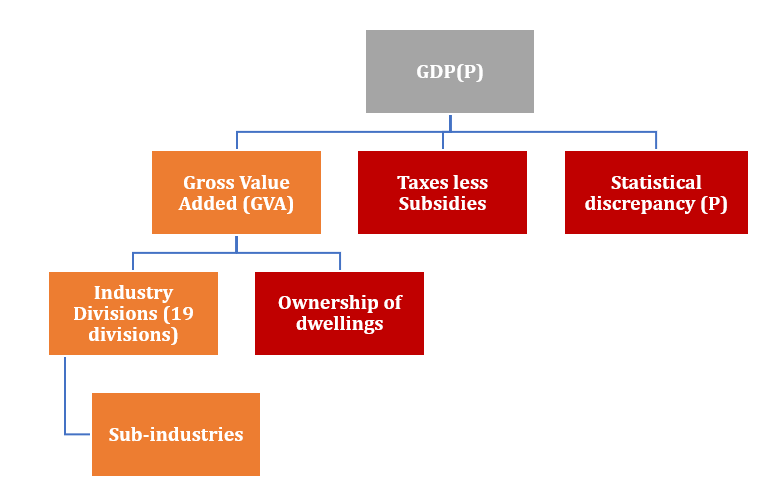
\includegraphics[scale=0.65]{Figs/GDP_P_fig1.PNG}
	\caption{Hierarchy of production approach.}\label{GDP_P_fig1}
\end{figure}

\begin{figure}[H]
	\centering
	\small
	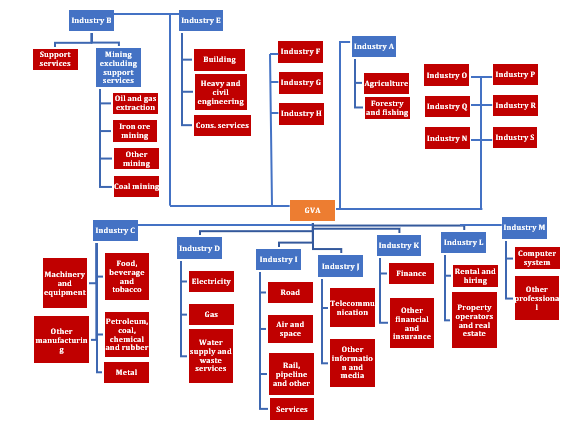
\includegraphics[scale=1]{Figs/GDP_P_fig2.PNG}
	\caption{Hierarchy of GVA under production approach.}\label{GDP_P_fig2}
\end{figure}

\begin{figure}[H]
	\centering
	\small
	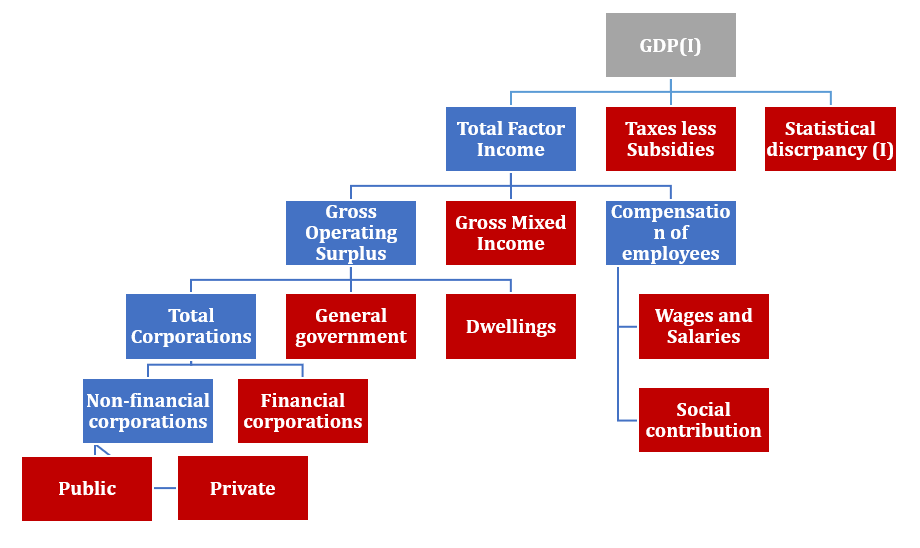
\includegraphics[scale=0.65]{Figs/GDP_I_fig1.PNG}
	\caption{Hierarchy of income approach.}\label{GDP_I_fig1}
\end{figure}

\begin{align*}
GDP(E) &= \textit{Final consumption expenditure} + \textit{Gross fixed capital formation} + \textit{Changes in inventories} +\\ &\textit{Exports of goods and services} - \textit{Imports of goods and services} + \textit{Statistical decrepency (E)}\\
\end{align*}
Associated hierarchical structure is given in figure \ref{GDP_E_fig1}, \ref{GDP_E_fig2} and \ref{GDP_E_fig3}.

\begin{figure}[H]
	\centering
	\small
	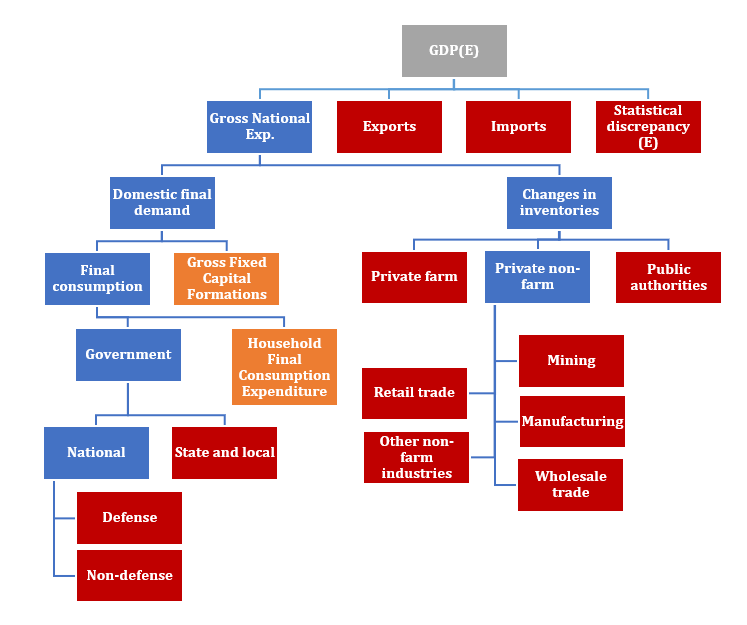
\includegraphics[scale=0.65]{Figs/GDP_E_fig1.PNG}
	\caption{Hierarchy of expenditure approach.}\label{GDP_E_fig1}
\end{figure}

\begin{figure}[H]
	\centering
	\small
	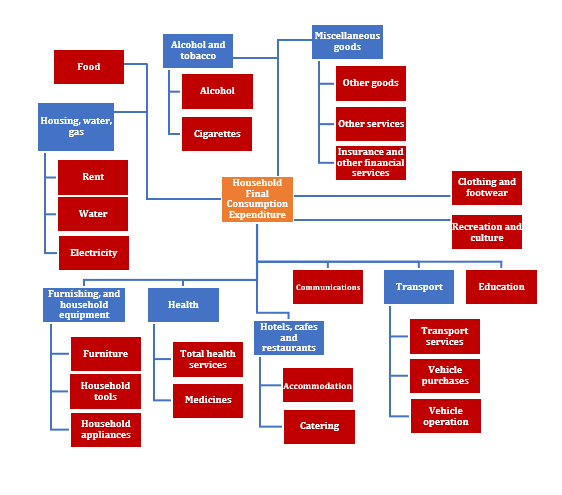
\includegraphics[scale=1]{Figs/GDP_E_fig2.PNG}
	\caption{Household final consumption expenditure under expenditure approach.}\label{GDP_E_fig2}
\end{figure}

\begin{figure}[H]
	\centering
	\small
	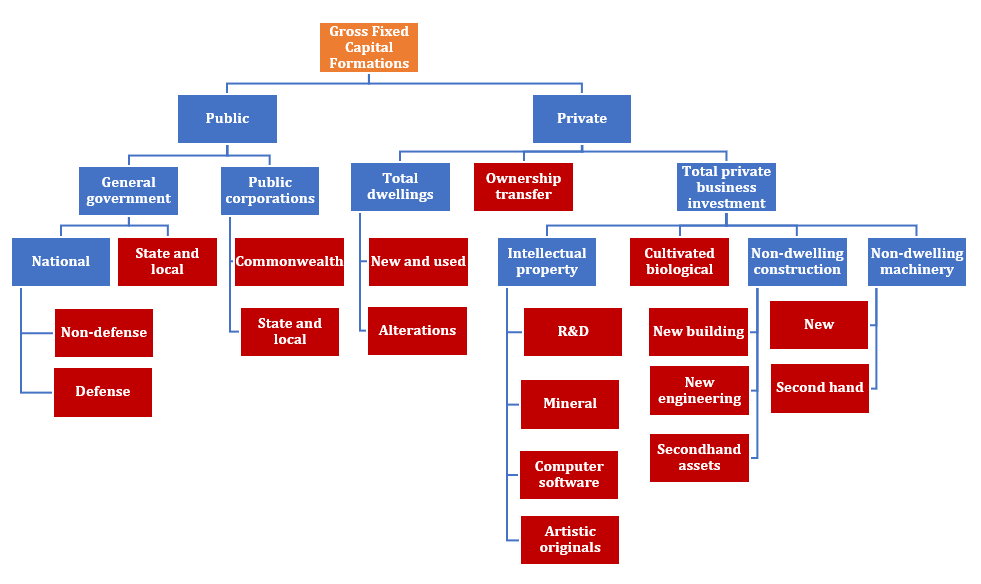
\includegraphics[scale=0.65]{Figs/GDP_E_fig3.PNG}
	\caption{Gross fixed capital formation (GFCF) under expenditure approach.}\label{GDP_E_fig3}
\end{figure}


\begin{table}[H] 
	\caption{Variables, Series IDs and their descriptions for Income Approach}
	\centering 
	\resizebox{\linewidth}{!}{
		\begin{tabular}[t]{lll}
			\toprule
			\textbf{Variable} & \textbf{Series ID} & \textbf{Description}\\
			\midrule
			Gdpi & A2302467A & GDP(I)\\
			Sdi & A2302413V & Statistical discrepancy (I)\\
			Tsi & A2302412T & Taxes less subsidies (I)\\
			TfiCoeWns & A2302399K & Compensation of employees; Wages and salaries\\
			TfiCoeEsc & A2302400J & Compensation of employees; Employers' social contributions\\
			\addlinespace
			TfiCoe & A2302401K & Compensation of employees\\
			TfiGosCopNfnPvt & A2323369L & Private non-financial corporations; Gross operating surplus\\
			TfiGosCopNfnPub & A2302403R & Public non-financial corporations; Gross operating surplus\\
			TfiGosCopNfn & A2302404T & Non-financial corporations; Gross operating surplus\\
			TfiGosCopFin & A2302405V & Financial corporations;  Gross operating surplus\\
			\addlinespace
			TfiGosCop & A2302406W & Total corporations; Gross operating surplus\\
			TfiGosGvt & A2298711F & General government; Gross operating surplus\\
			TfiGosDwl & A2302408A & Dwellings owned by persons; Gross operating surplus\\
			TfiGos & A2302409C & All sectors; Gross operating surplus\\
			TfiGmi & A2302410L & Gross mixed income\\
			Tfi & A2302411R & Total factor income\\
			\bottomrule
		\end{tabular}
		\label{Tab: Income-hierarchy}
	}
\end{table}

\begin{table}[H] 
	\caption{Variables, Series IDs and their descriptions for Expenditure Approach}
	\centering 
	\resizebox{\linewidth}{!}{
		\begin{tabular}[t]{lll}
			\toprule
			\textbf{Variable} & \textbf{Series ID} & \textbf{Description}\\
			\midrule
			
			Gdpe & A2302467A & GDP(E)\\
			Sde & A2302566J & Statistical Discrepancy(E)\\
			Exp & A2302564C & Exports of goods and services\\
			Imp & A2302565F & Imports of goods and services\\
			Gne & A2302563A & Gross national exp.\\
			\addlinespace
			GneDfdFceGvtNatDef & A2302523J & Gen. gov. - National; Final consumption exp. - Defence\\
			GneDfdFceGvtNatNdf & A2302524K & Gen. gov. - National; Final consumption exp. - Non-defence\\
			GneDfdFceGvtNat & A2302525L & Gen. gov. - National; Final consumption exp.\\
			GneDfdFceGvtSnl & A2302526R & Gen. gov. - State and local; Final consumption exp,\\
			GneDfdFceGvt & A2302527T & Gen. gov.; Final consumption exp.\\
			\addlinespace
			GneDfdFce & A2302529W & All sectors; Final consumption exp.\\
			GneDfdGfcPvtTdwNnu & A2302543T & Pvt.; Gross fixed capital formation (GFCF)\\
			GneDfdGfcPvtTdwAna & A2302544V & Pvt.; GFCF - Dwellings - Alterations and additions\\
			GneDfdGfcPvtTdw & A2302545W & Pvt.; GFCF - Dwellings - Total\\
			GneDfdGfcPvtOtc & A2302546X & Pvt.; GFCF - Ownership transfer costs\\
			\addlinespace
			GneDfdGfcPvtPbiNdcNbd & A2302533L & Pvt. GFCF - Non-dwelling construction - New building\\
			GneDfdGfcPvtPbiNdcNec & A2302534R & Pvt.; GFCF - Non-dwelling construction -\\
			&  & New engineering construction\\
			GneDfdGfcPvtPbiNdcSha & A2302535T & Pvt.; GFCF - Non-dwelling construction -\\
			&  & Net purchase of second hand \vphantom{1} assets\\
			\addlinespace
			GneDfdGfcPvtPbiNdc & A2302536V & Pvt.; GFCF - Non-dwelling construction - Total\\
			GneDfdGfcPvtPbiNdmNew & A2302530F & Pvt.; GFCF - Machinery and equipment - New\\
			GneDfdGfcPvtPbiNdmSha & A2302531J & Pvt.; GFCF - Machinery and equipment -\\
			&  & Net purchase of second hand assets\\
			GneDfdGfcPvtPbiNdm & A2302532K & Pvt.; GFCF - Machinery and equipment - Total\\
			\addlinespace
			GneDfdGfcPvtPbiCbr & A2716219R & Pvt.; GFCF - Cultivated biological resources\\
			GneDfdGfcPvtPbiIprRnd & A2716221A & Pvt.; GFCF - Intellectual property products -\\
			&  & Research and development\\
			GneDfdGfcPvtPbiIprMnp & A2302539A & Pvt.; GFCF - Intellectual property products -\\
			&  & Mineral and petroleum exploration\\
			\addlinespace
			GneDfdGfcPvtPbiIprCom & A2302538X & Pvt.; GFCF - Intellectual property products - Computer software\\
			GneDfdGfcPvtPbiIprArt & A2302540K & Pvt.; GFCF - Intellectual property products - Artistic originals\\
			GneDfdGfcPvtPbiIpr & A2716220X & Pvt.; GFCF - Intellectual property products Total\\
			GneDfdGfcPvtPbi & A2302542R & Pvt.;  GFCF - Total private business investment\\
			GneDfdGfcPvt & A2302547A & Pvt.; GFCF\\
			\addlinespace
			GneDfdGfcPubPcpCmw & A2302548C & Plc. corporations - Commonwealth; GFCF\\
			GneDfdGfcPubPcpSnl & A2302549F & Plc. corporations - State and local; GFCF\\
			GneDfdGfcPubPcp & A2302550R & Plc. corporations; GFCF Total\\
			GneDfdGfcPubGvtNatDef & A2302551T & Gen. gov. - National; GFCF - Defence\\
			GneDfdGfcPubGvtNatNdf & A2302552V & Gen. gov. - National ; GFCF - Non-defence\\
			\addlinespace
			GneDfdGfcPubGvtNat & A2302553W & Gen. gov. - National ; GFCF Total\\
			GneDfdGfcPubGvtSnl & A2302554X & Gen. gov. - State and local; GFCF\\
			GneDfdGfcPubGvt & A2302555A & Gen. gov.; GFCF\\
			GneDfdGfcPub & A2302556C & Plc.; GFCF\\
			GneDfdGfc & A2302557F & All sectors; GFCF\\
			\bottomrule
		\end{tabular}
		
		\label{Tab:Expenditure-hierarchy-1}
	}
\end{table}

\begin{table}[H] 
	\caption{Variables, Series IDs and their descriptions for Changes in Inventories - Expenditure Approach}
	\centering 
	\resizebox{\linewidth}{!}{
		\begin{tabular}[t]{lll}
			
			\toprule
			\textbf{Variable} & \textbf{Series ID} & \textbf{Description}\\
			\midrule
			
			GneCii & A2302562X & Changes in Inventories\\
			GneCiiPfm & A2302560V & Farm\\
			GneCiiPba & A2302561W & Public authorities\\
			GneCiiPnf & A2302559K & Private; Non-farm Total\\
			GneCiiPnfMin & A83722619L & Private; Mining (B)\\
			\addlinespace
			GneCiiPnfMan & A3348511X & Private; Manufacturing (C)\\
			GneCiiPnfWht & A3348512A & Private; Wholesale trade (F)\\
			GneCiiPnfRet & A3348513C & Private; Retail trade (G)\\
			GneCiiPnfOnf & A2302273C & Private; Non-farm; Other non-farm industries\\
			\bottomrule
		\end{tabular}
		\label{Tab:Expenditure-hierarchy-2}
	}
\end{table}

\begin{table}[H] 
	\caption{Variables, Series IDs and their descriptions for Household Final Consumption - Expenditure Approach}
	\centering 
	\resizebox{\linewidth}{!}{
		\begin{tabular}[t]{lll}
			
			\toprule
			\textbf{Variable} & \textbf{Series ID} & \textbf{Description}\\
			\midrule
			
			GneDfdHfc & A2302254W & Household Final Consumption Expenditure\\
			GneDfdFceHfcFud & A2302237V & Food\\
			GneDfdFceHfcAbt & A3605816F & Alcoholic beverages and tobacco\\
			GneDfdFceHfcAbtCig & A2302238W & Cigarettes and tobacco\\
			GneDfdFceHfcAbtAlc & A2302239X & Alcoholic beverages\\
			\addlinespace
			GneDfdFceHfcCnf & A2302240J & Clothing and footwear\\
			GneDfdFceHfcHwe & A3605680F & Housing, water, electricity, gas and other fuels\\
			GneDfdFceHfcHweRnt & A3605681J & Actual and imputed rent for housing\\
			GneDfdFceHfcHweWsc & A3605682K & Water and sewerage charges\\
			GneDfdFceHfcHweEgf & A2302242L & Electricity, gas and other fuel\\
			\addlinespace
			GneDfdFceHfcFhe & A2302243R & Furnishings and household equipment\\
			GneDfdFceHfcFheFnt & A3605683L & Furniture, floor coverings and household goods\\
			GneDfdFceHfcFheApp & A3605684R & Household appliances\\
			GneDfdFceHfcFheTls & A3605685T & Household tools\\
			GneDfdFceHfcHlt & A2302244T & Health\\
			\addlinespace
			GneDfdFceHfcHltMed & A3605686V & Medicines, medical aids and therapeutic appliances\\
			GneDfdFceHfcHltHsv & A3605687W & Total health services\\
			GneDfdFceHfcTpt & A3605688X & Transport\\
			GneDfdFceHfcTptPvh & A2302245V & Purchase of vehicles\\
			GneDfdFceHfcTptOvh & A2302246W & Operation of vehicles\\
			\addlinespace
			GneDfdFceHfcTptTsv & A2302247X & Transport services\\
			GneDfdFceHfcCom & A2302248A & Communications\\
			GneDfdFceHfcRnc & A2302249C & Recreation and culture\\
			GneDfdFceHfcEdc & A2302250L & Education services\\
			GneDfdFceHfcHcr & A2302251R & Hotels, cafes and restaurants\\
			\addlinespace
			GneDfdFceHfcHcrCsv & A3605694V & Catering services\\
			GneDfdFceHfcHcrAsv & A3605695W & Accommodation services\\
			GneDfdFceHfcMis & A3605696X & Miscellaneous goods and services\\
			GneDfdFceHfcMisOgd & A3605697A & Other goods\\
			GneDfdFceHfcMisIfs & A2302252T & Insurance and other financial services\\
			GneDfdFceHfcMisOsv & A3606485T & Other services\\
			\bottomrule
		\end{tabular}
		\label{Tab:Expenditure-hierarchy-3}
	}
\end{table}


\pagebreak
\bibliographystyle{agsm}

\bibliography{References_BookChapter_HTS}


\end{document}
